\documentclass{article}
\usepackage{graphicx} % Required for inserting images
\usepackage{qcircuit}
\usepackage{listings}

\usepackage{color}

\definecolor{dkgreen}{rgb}{0,0.6,0}
\definecolor{gray}{rgb}{0.5,0.5,0.5}
\definecolor{mauve}{rgb}{0.58,0,0.82}

\lstset{frame=tb,
  language=python,
  aboveskip=3mm, 
  belowskip=3mm,
  showstringspaces=false,
  columns=flexible,
  basicstyle={\scriptsize},
  frame={btlr},
  numbers=none,
  numberstyle=\tiny\color{gray},
  keywordstyle=\color{blue},
  commentstyle=\color{dkgreen},
  stringstyle=\color{mauve},
  breaklines=true,
  breakatwhitespace=true,
  tabsize=3
}

\title{CMPT 981 Mini Project}
\author{Marcus Edwards}
\date{March 2025}

\begin{document}

\maketitle

This was not my first exposure to Shor's algorithm, nor to coding parts of it. However, there were certainly components of this task which were firsts for me, such as implementing general modular exponentiation circuits, compiling to Clifford + T, and implementing phase estimation for more than three qubits.

In order to approach these tasks, I did some preliminary research. This led me to find the paper \cite{gamel2013simplifiedfactoringalgorithmsvalidating} which gives some examples of modular exponentiation circuits for use in Shor's algorithm. This paper builds these circuit straightforwardly from truth tables, for small numbers of qubits. For example, for the case where $N=21$, we have an input register of three qubits and $l=4$, the truth table is:

\begin{table}[h]
    \centering
    \begin{tabular}{|c  c  c  c  c  c  c  c  c|}
        \hline
        x & 0 & 1 & 2 & 3 & 4 & 5 & 6 & 7 \\
        \hline
        $4^x (mod \; 21)$ & 1 & 4 & 16 & 1 & 4 & 16 & 1 & 4 \\
        \hline
    \end{tabular}
    \caption{$f_{21,4}(x)$}
    \label{tab:my_label}
\end{table}

\vspace{5mm}

\begin{table}[h]
    \centering
    \begin{tabular}{|c  c  c  c  c  c  c  c|}
        \hline
        $x_2$ & $x_1$ & $x_0$ & $y_4$ & $y_3$ & $y_2$ & $y_1$ & $y_0$ \\
        \hline
        0 & 0 & 0 & 0 & 0 & 0 & 0 & 1 \\
        \hline
        0 & 0 & 1 & 0 & 0 & 1 & 0 & 0 \\
        \hline
        0 & 1 & 0 & 1 & 0 & 0 & 0 & 0 \\
        \hline
        0 & 1 & 1 & 0 & 0 & 0 & 0 & 1 \\
        \hline
        1 & 0 & 0 & 0 & 0 & 1 & 0 & 0 \\
        \hline
        1 & 0 & 1 & 1 & 0 & 0 & 0 & 0 \\
        \hline
        1 & 1 & 0 & 0 & 0 & 0 & 0 & 1 \\
        \hline
        1 & 1 & 1 & 0 & 0 & 1 & 0 & 0 \\
        \hline
    \end{tabular}
    \caption{$f_{21,4}(x)$ Truth Table}
    \label{tab:my_label}
\end{table}

\vspace{5mm}

The correspoding circuit is provided, in terms of Xs, CNOTs and Toffolis. As an example to myself, I was easily able to implement this circuit using Xanadu's Pennylane.

\begin{figure}[h]
    \[
        \begin{array}{c}
            \Qcircuit @C=1em @R=.7em {
                \lstick{x_2}     & \qw & \qw & \qw & \ctrl{7} & \qw & \ctrl{7} & \qw & \ctrl{7} & \qw & \qw & \ctrl{5} & \qw & \qw & \ctrl{7} \\
                \lstick{x_1}     & \ctrl{4} & \qw & \ctrl{6} & \qw & \qw & \qw & \ctrl{6} & \qw & \qw & \qw & \qw & \qw & \ctrl{6} & \qw \\
                \lstick{x_0}     & \qw & \ctrl{3} & \qw & \qw & \qw & \qw & \qw & \qw & \qw & \qw & \qw & \ctrl{5} & \qw & \qw \\
                \lstick{\ket{0}} & \qw & \qw & \qw & \qw & \targ & \qw & \qw & \ctrl{4} & \ctrl{2} & \qw & \qw & \qw & \qw & \qw \\
                \lstick{\ket{0}} & \qw & \qw & \qw & \qw & \qw & \qw & \qw & \qw & \qw & \qw & \qw & \qw & \qw & \qw \\
                \lstick{\ket{0}} & \targ & \targ & \qw & \qw & \ctrl{-2} & \qw & \qw & \qw & \targ & \targ & \targ & \qw & \qw & \qw \\
                \lstick{\ket{0}} & \qw & \qw & \qw & \qw & \qw & \qw & \qw & \qw & \qw & \qw & \qw & \qw & \qw & \qw \\
                \lstick{\ket{0}} & \qw & \qw & \targ & \targ & \ctrl{-4} & \targ & \targ & \targ & \qw & \ctrl{-2} & \targ & \targ & \targ & \targ \\
            }
        \end{array}
    \]
    \caption{\centering $f_{21,4}(x)$ Circuit}
\end{figure}

\vspace{5mm}

\begin{lstlisting}
    @qml.qnode(dev)
    def f_21_4():
        qml.CNOT([1, 5])
        qml.CNOT([2, 5])
        qml.CNOT([1, 7])
        qml.CNOT([0, 7])
        qml.Toffoli([7, 5, 3])
        qml.CNOT([0, 7])
        qml.CNOT([1, 7])
        qml.Toffoli([0, 3, 7])
        qml.CNOT([3, 5])
        qml.CNOT([7, 5])
        qml.PauliX(7)
        qml.CNOT([0, 5])
        qml.CNOT([2, 7])
        qml.CNOT([1, 7])
        qml.CNOT([0, 7])
\end{lstlisting}

Through this exercise it became clear to me that these circuits could be synthesized from truth tables. The linear transformation corresponding to such a truth table can be solved for programmatically. This is akin to solving a linear system of equations with binary variables.

Since there was a prize to be won for the most efficient circuit in terms of T count, I thought there was reason to include an exhaustive search for solutions besides the known Cuccaro ripple carry adder approach. To this end, I wrote a function which would attempt to solve for in-place and then out-of-place linear transformations by brute force which might(?) be more efficient implementations of the modular exponentiation unitaries than the formulaic ripple-carry adder approach which works in all cases but is not optimized for any particular modular exponentiation circuit.

Some challenges arose as I wrote this part of the implementation. Namely, Python's Numpy can solve linear systems of equations with `linalg.solve`, but since the modular exponentiation functions' truth tables yielded underdetermined systems, there were an infinite number of solutions and this approach was not viable. Neither was `linalg.lstsq`, which returns the least-squares solution, viable since even this solution was not possible to constrain to solve for binary values only. Matlab has a function for solving linear systems of binary variables, but Python does not.

Therefore, I wrote my own solution for solving for these linear transformations. This is inefficient, however the approach should be accurate. Hopefully, using the approach in \cite{patel_efficient_2003} to then synthesize CNOT circuits from these linear transformations efficiently offsets the inefficiency of solving for these transformations in the first place.

There were several challenges implementing the algorithm for efficient circuit synthesis presented in \cite{patel_efficient_2003}. The pseudocode in the paper uses some language features which are not present in Python. For example, tensors (ranges of values representing the patterns found in the sub-rows) are used as array indices. Tensors in Numpy are unhashable types. Therefore, I had to implement a hashing function for these. I chose to convert the individual entries into strings up to a certain precision and concatenate them. 

\begin{lstlisting}
def hash_pattern(arr, precision=10):
    """
    Hashes a sub-row pattern.
    :param arr: The sub-row pattern.
    :param precision: The float precision up to which to maintain uniqueness between tensors.
    :return: The hash.
    """
    hash = ''
    if arr.shape == ():
        return str(arr)
    for elem in arr:
        if not isinstance(elem, np.tensor) and not isinstance(elem, np.ndarray) and not isinstance(elem, list):
            hash += str(elem).split('.')[0] + '.'
            if len(str(elem).split('.')) > 1:
                dec = str(elem).split('.')[1]
                i = 0
                while i < len(dec) and i < precision:
                    hash += dec[i]
                    i += 1
        else:
            hash += hash_pattern(elem, precision)
    return hash 
\end{lstlisting}

I also had to translate the tuples which represent CNOTs in \cite{patel_efficient_2003} into Pennylane circuits.

\begin{lstlisting}
# convert to pennylane circuit
for j in range(len(circuit)):
    compileMultiControlledX(wires=(c, circuit[j][0] + INPUT_QUBITS, circuit[j][1] + INPUT_QUBITS),)
\end{lstlisting}

This is where two further considerations came into the picture. Instead of simply converting each tuple (control, target) into a CNOT gate, I added the appropriate extra control to make a Toffoli so that each entire modular exponentiation circuit was controlled by the appropriate qubit in the input register. Next, I compiled each Toffoli to Clifford + T using the compilation specified in \cite{welch_efficient_2015}.

\begin{figure}[h!]
    \centering
    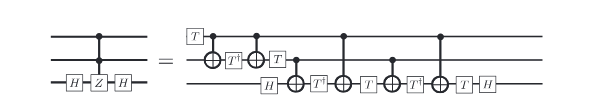
\includegraphics[width=1\linewidth]{circuit.png}
\end{figure}

\begin{lstlisting}
def compileMultiControlledX(wires):
    """
    Compile a Toffoli to Clifford+T using the approach in:

    [1] J. Welch, A. Bocharov, and K. Svore, “Efficient Approximation of
    Diagonal Unitaries over the Clifford+T Basis,” Quantum information & computation,
    vol. 16, Dec. 2014, doi: 10.26421/QIC16.1-2-6.

    :param wires: The wires the gate acts on, with the target wire last.
    :return:
    """
    qml.T(wires=wires[0])
    qml.CNOT(wires=(wires[0], wires[1]))
    qml.adjoint(qml.T(wires=wires[1]))
    qml.CNOT(wires=(wires[0], wires[1]))
    qml.T(wires=wires[1])
    qml.H(wires=wires[2])
    qml.CNOT(wires=(wires[1], wires[2]))
    qml.adjoint(qml.T(wires=wires[2]))
    qml.CNOT(wires=(wires[0], wires[2]))
    qml.T(wires=wires[2])
    qml.CNOT(wires=(wires[1], wires[2]))
    qml.adjoint(qml.T(wires=wires[2]))
    qml.CNOT(wires=(wires[0], wires[2]))
    qml.T(wires=wires[2])
    qml.H(wires=wires[2])
\end{lstlisting}

When these methods failed, the default approach using the Cuccaro ripple carry adder was used. The building of the Cuccaro adder was implemented recursively, evaluating one addition in the sum $(((a_0^{2^i} b + a_1^{2^i} 2b) + a_2^{2^i} 2^2 b) + \dots + a_{n-1}^{2^i} 2^{n-1} b)$ per function call, where the scope of the evaluation in each stack frame is denoted by the brackets. The value $b$ was persisted in an ancilla register, and the shifting was done by adding $b$ to the most significant $n - j$ bits of the output register, where $j$ is the subscript on the $a_j^{2^i}$ and the amount of the shift. 


\begin{lstlisting}
def build_adder_circuit(a, c):
    """
    Builds a circuit to do modular multiplication via shifted additions.
    :param a: The pre-calculated l**(2**i).
    :param c: The controlling qubit.
    :return:
    """
    n = OUTPUT_QUBITS
    shift = 0  # not the i in the docstring... this one indexes a's bits

    # load b into ancilla register
    for j in range(OUTPUT_QUBITS):
        compileMultiControlledX((c, INPUT_QUBITS + j, INPUT_QUBITS + OUTPUT_QUBITS + j))

    assert build_adder_circuit_helper(format(int(a), '#07b').split('b')[1][::-1], n, shift, c)


def build_adder_circuit_helper(a, n, shift, c):
    """
    Recursive function that builds the modular multiplication circuit with shifted additions.
    :param a: The pre-calculated l**(2**j) as a big endian binary string.
    :param n: The size of the registers.
    :param i: The current index (from least to most significant digits).
    :param c: The controlling qubit.
    :return: whether finished.
    """
    if shift == n:
        return True
    elif shift == 0:
        if bool(a[shift]) is False:
            # reset output register
            for j in range(OUTPUT_QUBITS):
                qml.measure(INPUT_QUBITS + j, reset=True)
        return build_adder_circuit_helper(a, n, shift + 1, c)
    else:
        if bool(a[shift]) is True:

            # add shifted b to the output register
            carry_qubit = INPUT_QUBITS + OUTPUT_QUBITS + ANCILLA_QUBITS + 0
            output_qubit = INPUT_QUBITS + 0 + shift
            ancilla_qubit = INPUT_QUBITS + OUTPUT_QUBITS + 0

            MAJ((carry_qubit, output_qubit, ancilla_qubit), c)

            for _ in range(1 + shift, OUTPUT_QUBITS):
                carry_qubit = ancilla_qubit
                output_qubit = output_qubit + 1
                ancilla_qubit = ancilla_qubit + 1

                MAJ((carry_qubit, output_qubit, ancilla_qubit), c)

            carry_output_qubit = INPUT_QUBITS + OUTPUT_QUBITS + ANCILLA_QUBITS + 1
            compileMultiControlledX((c, ancilla_qubit, carry_output_qubit))

            UMA((carry_qubit, output_qubit, ancilla_qubit), c)

            for _ in range(OUTPUT_QUBITS - 1, shift, -1):
                ancilla_qubit = carry_qubit
                output_qubit = output_qubit - 1
                carry_qubit = carry_qubit - 1
                UMA((carry_qubit, output_qubit, ancilla_qubit), c)
        return build_adder_circuit_helper(a, n, shift + 1, c)

\end{lstlisting}


Some challenges associated with this implementation were the need to have the entire thing controlled by an input qubit, needing sometimes to be able to reset the output qubit register when the bit of least significance in the $a^{2^i}$ term was zero, and the sheer number of indices to keep track of in the implementation. Of course, there was also the challenge of needing to read multiple technical papers to understand this approach in the first place.

To address the first of these challenges, Python's partial function from the functools library was used in various places to pre-initialize and re-package functions which built Pennylane circuits into functions which would take a controlling qubit index as a sole parameter and then implement the entire circuit with an extra control on each CNOT, Toffoli, X, etc. This was to allow the control of the entire modular multiplication unitary by an input qubit line. The mid-circuit reset feature of Pennylane was sued to address the second of the challenges, but this has limitations. Namely, the reset works by provisioning an entire new register and so it can make the number of qubits blow up. The challenges with keeping track of indices etc. was done by the use of careful naming and commenting conventions. In particular, it was important to remember that binary values were indexed from least to most significant bit in the Cuccaro paper. Therefore, when iterating over binary values, it was sometimes necessary to reverse them to match what was in the corresponding qubit register.
A final challenge was that the circuit ended up so large that Python's max allowed recursion depth needed to be extended in order to print it.

This approach yielded a very large circuit, and counting Ts by hand was arduous. Therefore, I printed the circuit to a file and used grep to count the occurences of the word ``T''. This yielded 1812. Next was to count the number of single qubit rotations and multiply it by $3 log_2(1/\epsilon)$. This yielded $1404 \times 3 log_2(1/10^{-7})$. It adds up for a total of 99756 T gates.

My code was able to successfully factor 32 into 4 and 8. It was tried with both the QFT and adjoint of QFT at the end of the circuit, which are both valid since it is the period of the peaks in measurement outcome probability which we care about. Getting the code to work required a lot of debugging and problem solving. Debugging the circuit directly would be a difficult task since it is so large, but it was easier to inspect and verify the function of the individual parts such as the modular exponentiation unitaries. This was done prior to the compilation to Clifford + T to make it easier. To this end, and to make our work easier to grade, the circuit was generated with and without compilation to Clifford + T.

\bibliographystyle{alpha}
\bibliography{biblio}

\end{document}
